% TEX compiler = luatex
% copyright arturo salinas-aguayo 2025
\documentclass[12pt]{article}

\usepackage{graphicx}
\usepackage{subcaption}
\usepackage{amsmath}
\usepackage{array}
\usepackage{amsfonts}
\usepackage{fancyhdr}
\usepackage{geometry}
\usepackage{circuitikz}
\usepackage{subfigure}
\usepackage{caption}
\usepackage{karnaugh-map}
\usepackage{bm}
\usepackage{float}

\geometry{letterpaper, margin=1in}
\graphicspath{ {../../images/} }

% Header and Footer
\pagestyle{fancy}
\fancyhf{}
\fancyhead[L]{ECE 2001 - Lab 06: Passive Filter Circuits}
\fancyhead[R]{\thepage}
\setlength{\headheight}{15pt}

\author{Arturo Salinas-Aguayo}
\title{Lab 006: Passive Filter Circuits}

% theorem set
\newtheorem{example}{Example}
% Example block environment
\newenvironment{examp}
{\vspace{0.5cm}
 \hrule
\vspace{0.5cm}
\begin{example}}
{\hrule
\vspace{0.5cm}
\end{example}}

\begin{document}
\newcommand{\closure}[2][3]{%
	{}\mkern#1mu\overline{\mkern-#1mu#2}}
\newcommand\ncoverline[1]{\mkern1mu\overline{\mkern-1mu#1\mkern-1mu}\mkern1mu}
% Title Page
\begin{titlepage}
	\centering
	\vspace*{3cm}
	\huge\textbf{Lab 06: Passive Filter Circuits}\\
	
	\vspace{5cm}
	\Large\textbf{Arturo Salinas-Aguayo}\\
	\normalsize
	ECE 2001 Electrical Circuits\\
	Dr. David J. Giblin, Section 331.660.701.810-1253\\
	Mechanical Engineering Department
	\vfill
	
\includegraphics[scale=0.1]{uconnlogo}\\
	College of Engineering, University of Connecticut\\
	\scriptsize{Coded in \LaTeX}
	\vspace*{1cm}
\end{titlepage}
\tableofcontents
\newpage
\section{Abstract}
This lab introduces frequency domain behavior of passive filters composed of resistors, capacitors, and inductors. Through experimentation with low-pass and high-pass filters, as well as an underdamped RLC configuration, the frequency response and phase shift characteristics are observed. Emphasis is placed on understanding cutoff frequency, amplitude response, and the resonance phenomenon.

\newpage
\section{Introduction}
While earlier labs focused on transient response, this experiment shifts the focus to the steady-state sinusoidal behavior of filters. The goal is to understand how the amplitude and phase of a circuit’s output vary as a function of frequency. By examining first-order filters and a second-order resonant circuit, intuition is built for applications in audio electronics, communication systems, and signal processing.

Filters are circuits that selectively allow or reject certain frequencies. Low-pass filters allow low frequencies to pass while attenuating higher ones. High-pass filters do the opposite. The transition point between passing and attenuation is the cutoff frequency, defined where the output amplitude is $\frac{1}{\sqrt{2}}$ of the input.

\section{Theory}
\subsection{Low-Pass RC Filter}
A first-order RC low-pass filter has the following configuration:


The transfer function is:
\[
	H(f) = \frac{1}{1 + j2\pi fRC}
\]
The cutoff frequency is given by:
\[
	f_c = \frac{1}{2\pi RC}
\]

\subsection{High-Pass RC Filter}
A high-pass RC filter simply swaps the resistor and capacitor:


The transfer function becomes:
\[
	H(f) = \frac{j2\pi fRC}{1 + j2\pi fRC}
\]
With the same cutoff frequency:
\[
	f_c = \frac{1}{2\pi RC}
\]

\subsection{Second-Order RLC Circuit (Bandpass Filter)}
An underdamped RLC circuit exhibits resonance. The circuit is:


Its transfer function peaks at:
\[
	f_0 = \frac{1}{2\pi\sqrt{LC}} \quad \text{(resonant frequency)}
\]
And has a quality factor $Q$:
\[
	Q = \frac{1}{R} \sqrt{\frac{L}{C}}
\]

\section{Experimental Procedures}
\subsection{Circuit One: RC High-Pass Filter}
A high pass filter is formed when the output of an RC circuit is taken off the
resistor. 
Cutoff Frequency - 
\begin{figure}[H]
	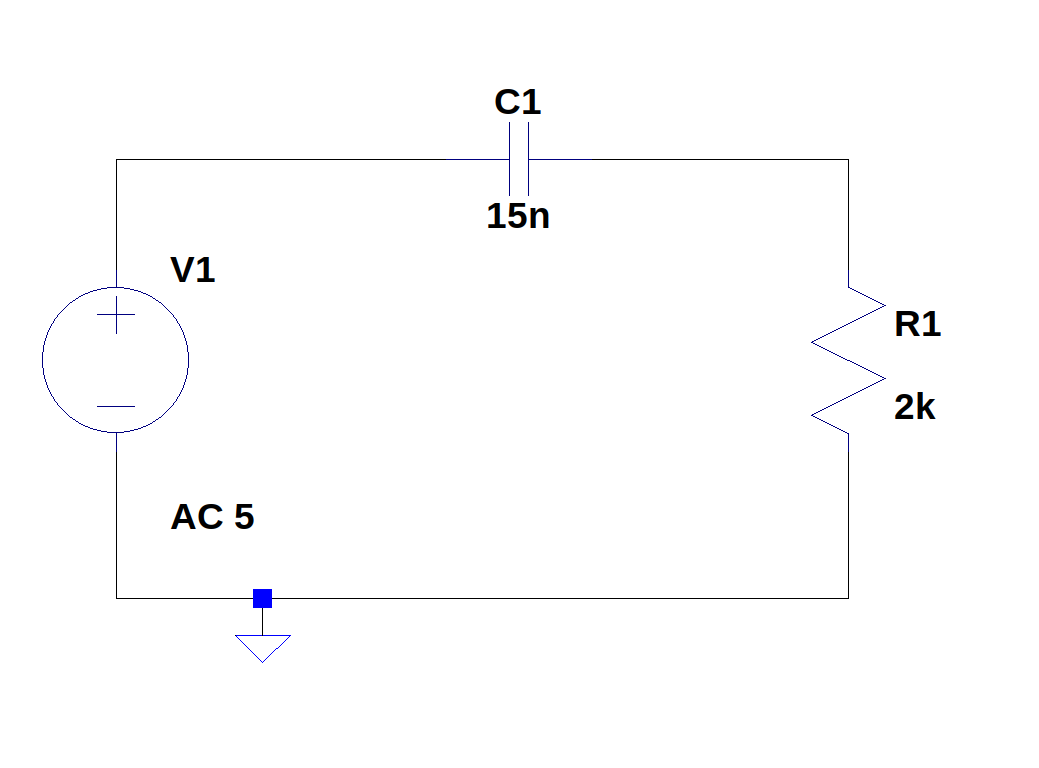
\includegraphics[width=\textwidth]{e6_01}
\end{figure}

\begin{itemize}
	\item Input signal: $5\,\mathrm{V_{pp}}$ sine wave
	\item Frequency sweep: $1\,\mathrm{Hz}$ to $100\,\mathrm{MHz}$
	\item Measure amplitude and phase of output across resistor.
\end{itemize}

\subsection{Circuit Two: RC Low-Pass Filter}
A typical low-pass filter is formed when the output of an RC circuit is taken
off the capacitor.

\begin{figure}[H]
	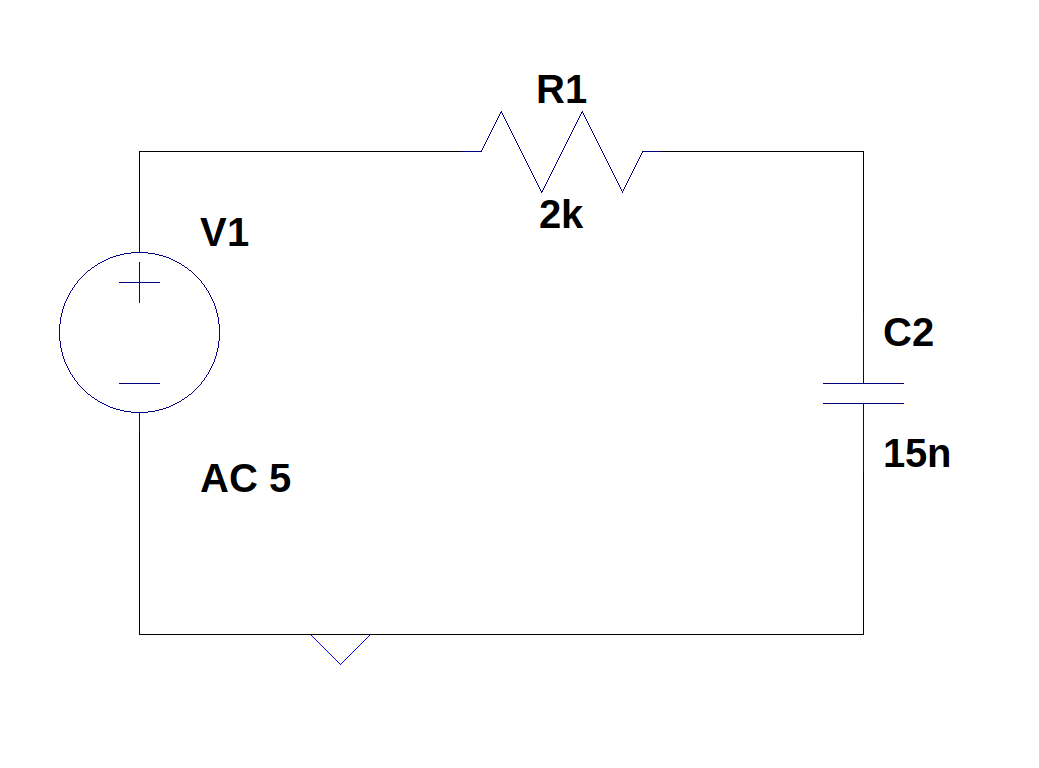
\includegraphics[width=\textwidth]{e6_02}
\end{figure}
\begin{itemize}
	\item Same input signal and frequency sweep
	\item Measure output across capacitor
\end{itemize}

\subsection{Circuit Three: Parallel Capacitor Low Pass Filter}

\begin{figure}[H]
	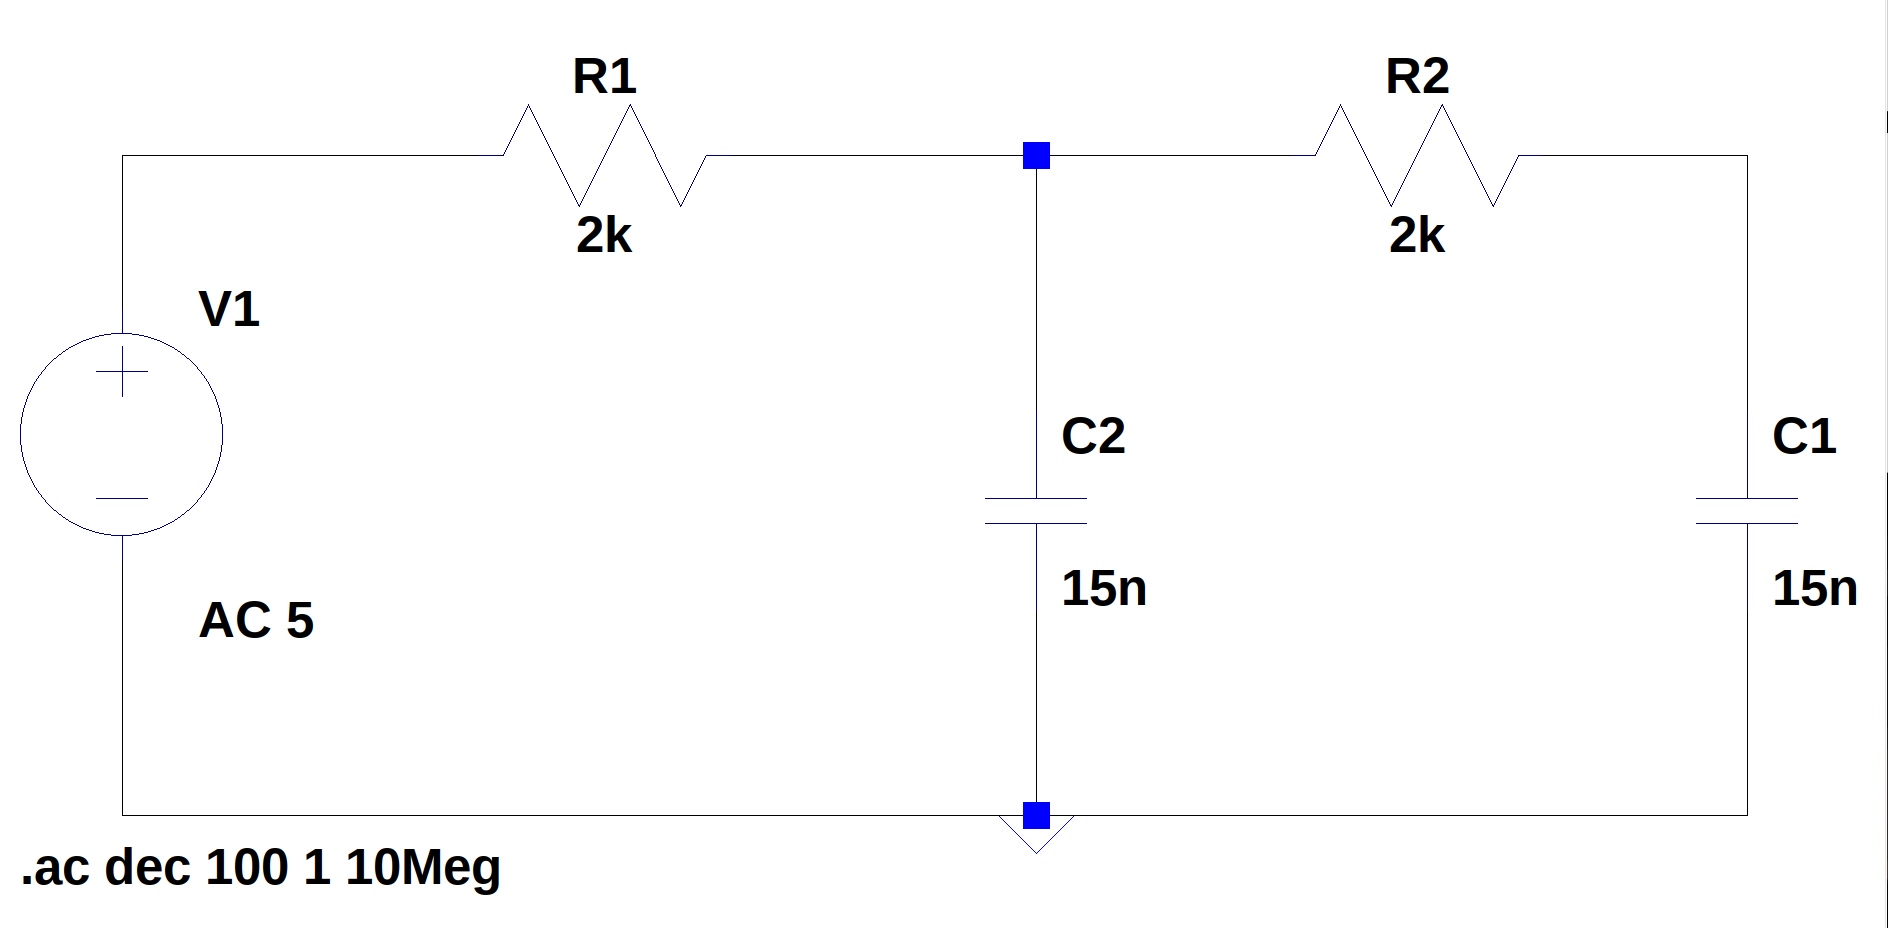
\includegraphics[width=\textwidth]{e6_03}
\end{figure}
\begin{itemize}
	\item Determine resonant frequency and bandwidth
	\item Plot Bode plot of magnitude response
\end{itemize}
\subsection{Circuit Four Series RLC Bandpass Filter}

\begin{figure}[H]
	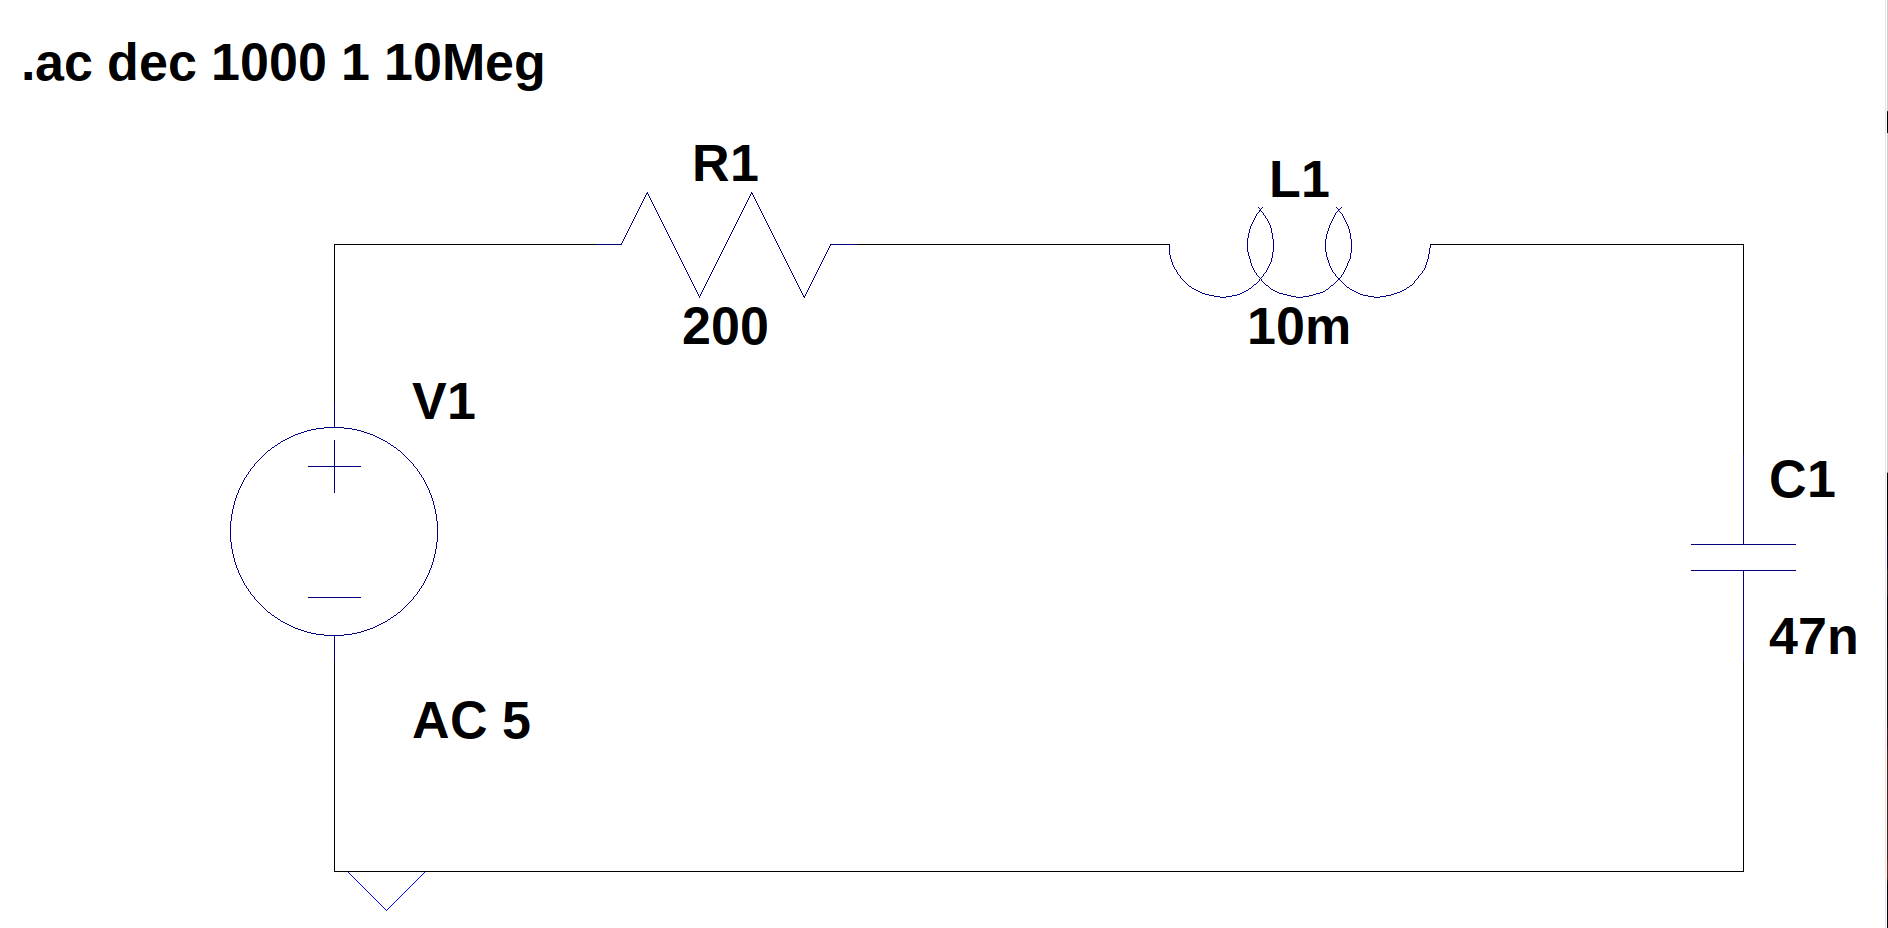
\includegraphics[width=\textwidth]{e6_04}
\end{figure}
\begin{itemize}
	\item Determine resonant frequency and bandwidth
	\item Plot Bode plot of magnitude response
\end{itemize}

\section{Results and Discussion}
\subsection{Low-Pass Filter Analysis}
[Insert oscilloscope and simulation images]
\begin{itemize}
	\item Compare theoretical cutoff with measured
	\item Plot amplitude response and extract $-3\,\mathrm{dB}$ point
\end{itemize}

\subsection{High-Pass Filter Analysis}
[Insert oscilloscope and simulation images]
\begin{itemize}
	\item Same analysis as low-pass
	\item Note phase shift at low frequencies
\end{itemize}

\subsection{RLC Resonant Filter}
[Insert scope screenshots and LTSpice waveform]
\begin{itemize}
	\item Compare calculated resonant frequency with observed
	\item Discuss the role of $Q$ and peak amplitude
\end{itemize}

\section{Conclusion}
This lab demonstrated the role of passive filters in shaping the frequency content of signals. First-order filters showed characteristic $-20\,\mathrm{dB/decade}$ roll-off near cutoff, while the second-order RLC circuit showed clear resonant behavior. Agreement between theory, simulation, and measurement confirms the behavior of these filters and prepares students for future work in frequency-selective networks and analog signal processing.
\end{document}
% vim: set ft=tex tw=80 ts=2 sts=2 sw=2 noet spell:
